\chapter{Anforderungen}
\label{ch:requirements}
In diesem Kapitel werden die Anforderungen für den im vorherigen Kapitel aufgezeigten Anwendungsfall aufgestellt. Dazu werden zunächst einige Standards vorgestellt, wie Anforderungen klassifiziert und eingeordnet werden können. Diese Standards werden anschließend in einem angepassten Modell zusammengeführt und auf die konkreten Anforderungen angewandt. Abschließend werden alle typisierten Anforderungen auf \ac{DLT}-Relevanz geprüft und schrittweise reduziert, um letztlich diejenigen Anforderungen sowie deren Klassen zu identifizieren, die für die Umsetzung auf einer \ac{DLT}-basierten Lösung entscheidend sind.

%
% Section: Standards und Normen
%
\section{Standards und Normen}
\label{sec:requirements:standards}
In diesem Abschnitt werden die verwendeten Standards und Normen aufgelistet und kurz beschrieben:
\begin{description}
  \item[BABOK] Das \ac{BABOK} wird vom \ac{IIBA} herausgegeben und stellt einen Leitfaden für die Business-Analyse dar, genauere Informationen können \cite{BABOK} entnommen werden. Es unterteilt in sogenannte Knowledge-Areas und vermittelt Techniken und Kompetenzen im Umfeld der Business-Analyse. Anforderungen werden im \ac{BABOK} nach Abstraktionsebene gruppiert: Die Business-Ebene, die Anforderungen abstrakt aus Sicht der gesamten Organisation betrachtet, die Stakeholder-Ebene, die die Anforderungen aus Sicht der verschiedenen Stakeholder beschreibt und die Solution-Ebene, die in funktionale und nicht-funktionale Anforderungen unterscheidet. Darüber hinaus gibt es eine Transition-Ebene, die temporäre Übergangsanforderungen zwischen dem Ausgangs- und dem Zielzustand des Gesamtsystems beschreibt.
  \item[PMBOK]  Das \ac{PMBOK} wird vom \ac{PMI} herausgegeben und ist der State-of-the-Art Standard im Bereich Projektmanagement, siehe \cite{PMBOK}. Das Werk teilt seine Sektionen ebenfalls wie das \ac{BABOK} in sogenannte Knowledge-Areas ein und kennt die gleiche Gruppierung im Bereich Anforderungsmanagement. Neben der Einteilung in Business, Stakeholder, Solution und Transition kennt das \ac{PMBOK} noch Quality und Project Anforderungen.
  \item[SWEBOK] \cite{SWEBOK} \ac{SWEBOK}
  \item[SEBOK] \cite{SEBOK} \ac{SEBOK}
  \item[ISO29148] \cite{ISO29148} \ac{ISO} 29148
  \item[ISO25010] \cite{ISO25010} \ac{ISO} 25010
\end{description}
Das Schaubild \ref{fig:chapter05:requirements} zeigt die unterschiedlichen Normen und Standards grafisch auf und stellt die verschiedenen Anforderungsgruppierungen zueinander in Beziehung.

\begin{figure}[htbp]
 \centering
 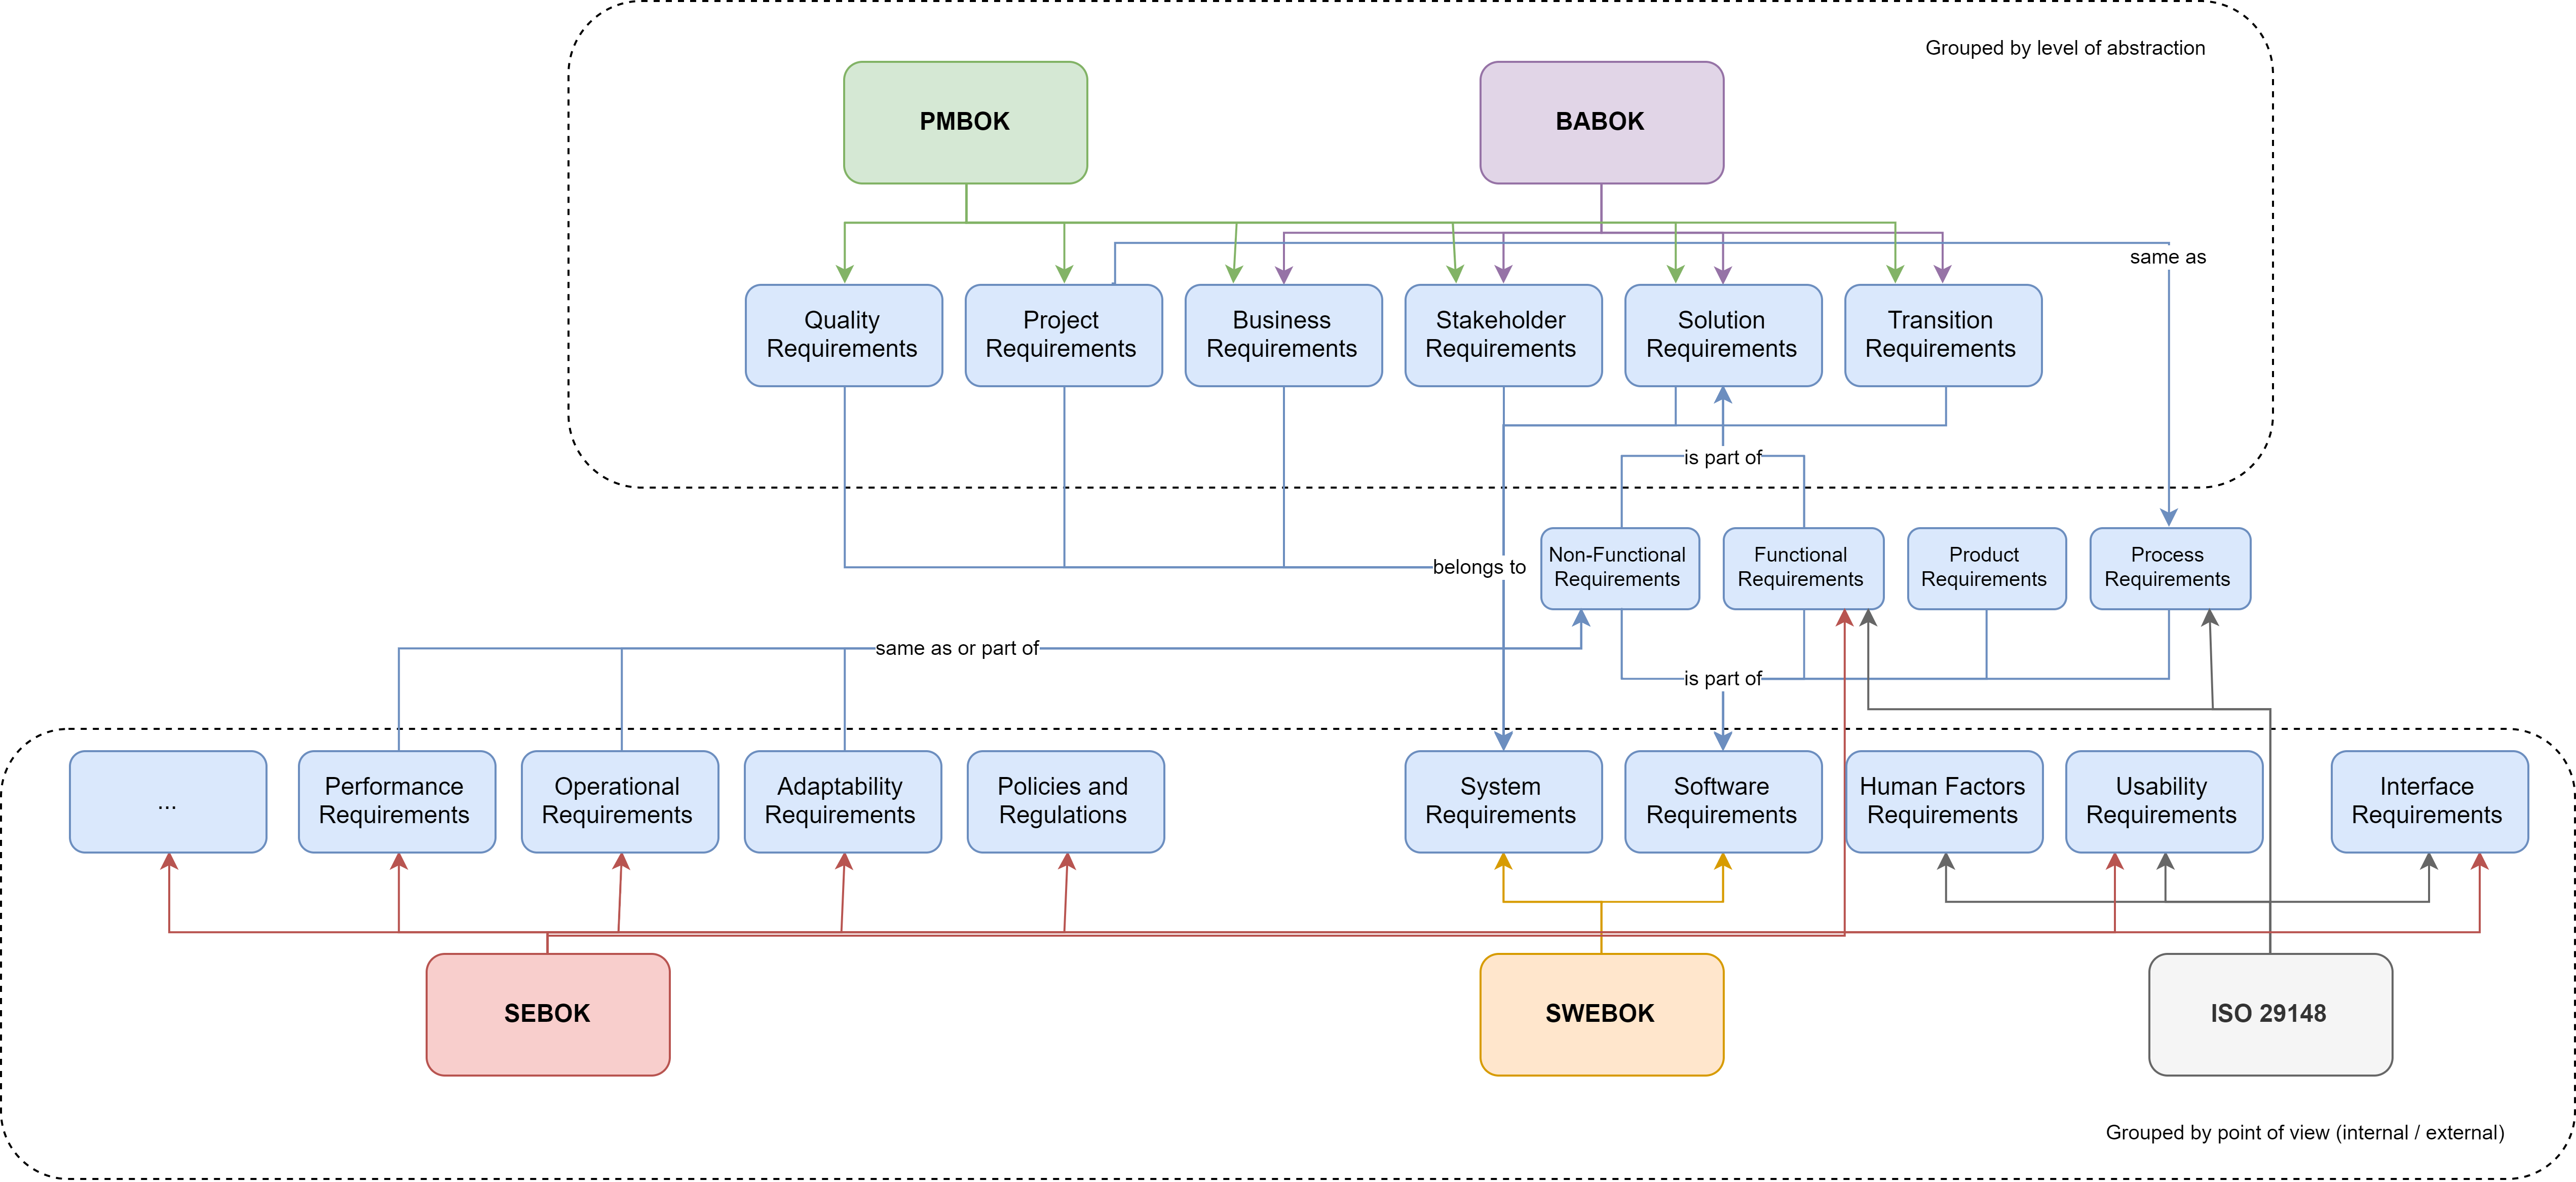
\includegraphics[width=1.0\textwidth]{gfx/Requirements.png}
 \caption{Einordnung der Begriffe und Zusammenhänge unterschiedlicher Normen und Standards}
 \label{fig:chapter05:requirements}
\end{figure}

Grundsätzlich unterscheiden die vorgestellten Ansätze zur Anforderungsklassifizierung in zwei Sichtweisen: \ac{PMBOK} und \ac{BABOK} unterscheiden Anforderungen nach Abstraktionslevel während \ac{SWEBOK}, \ac{SEBOK} und ISO29148 primär nach der Perspektive der Stakeholder gruppieren. Das Schaubild \ref{fig:chapter05:requirements_grouping} stellt diesen Zusammenhang grafisch dar.

\begin{figure}[htbp]
 \centering
 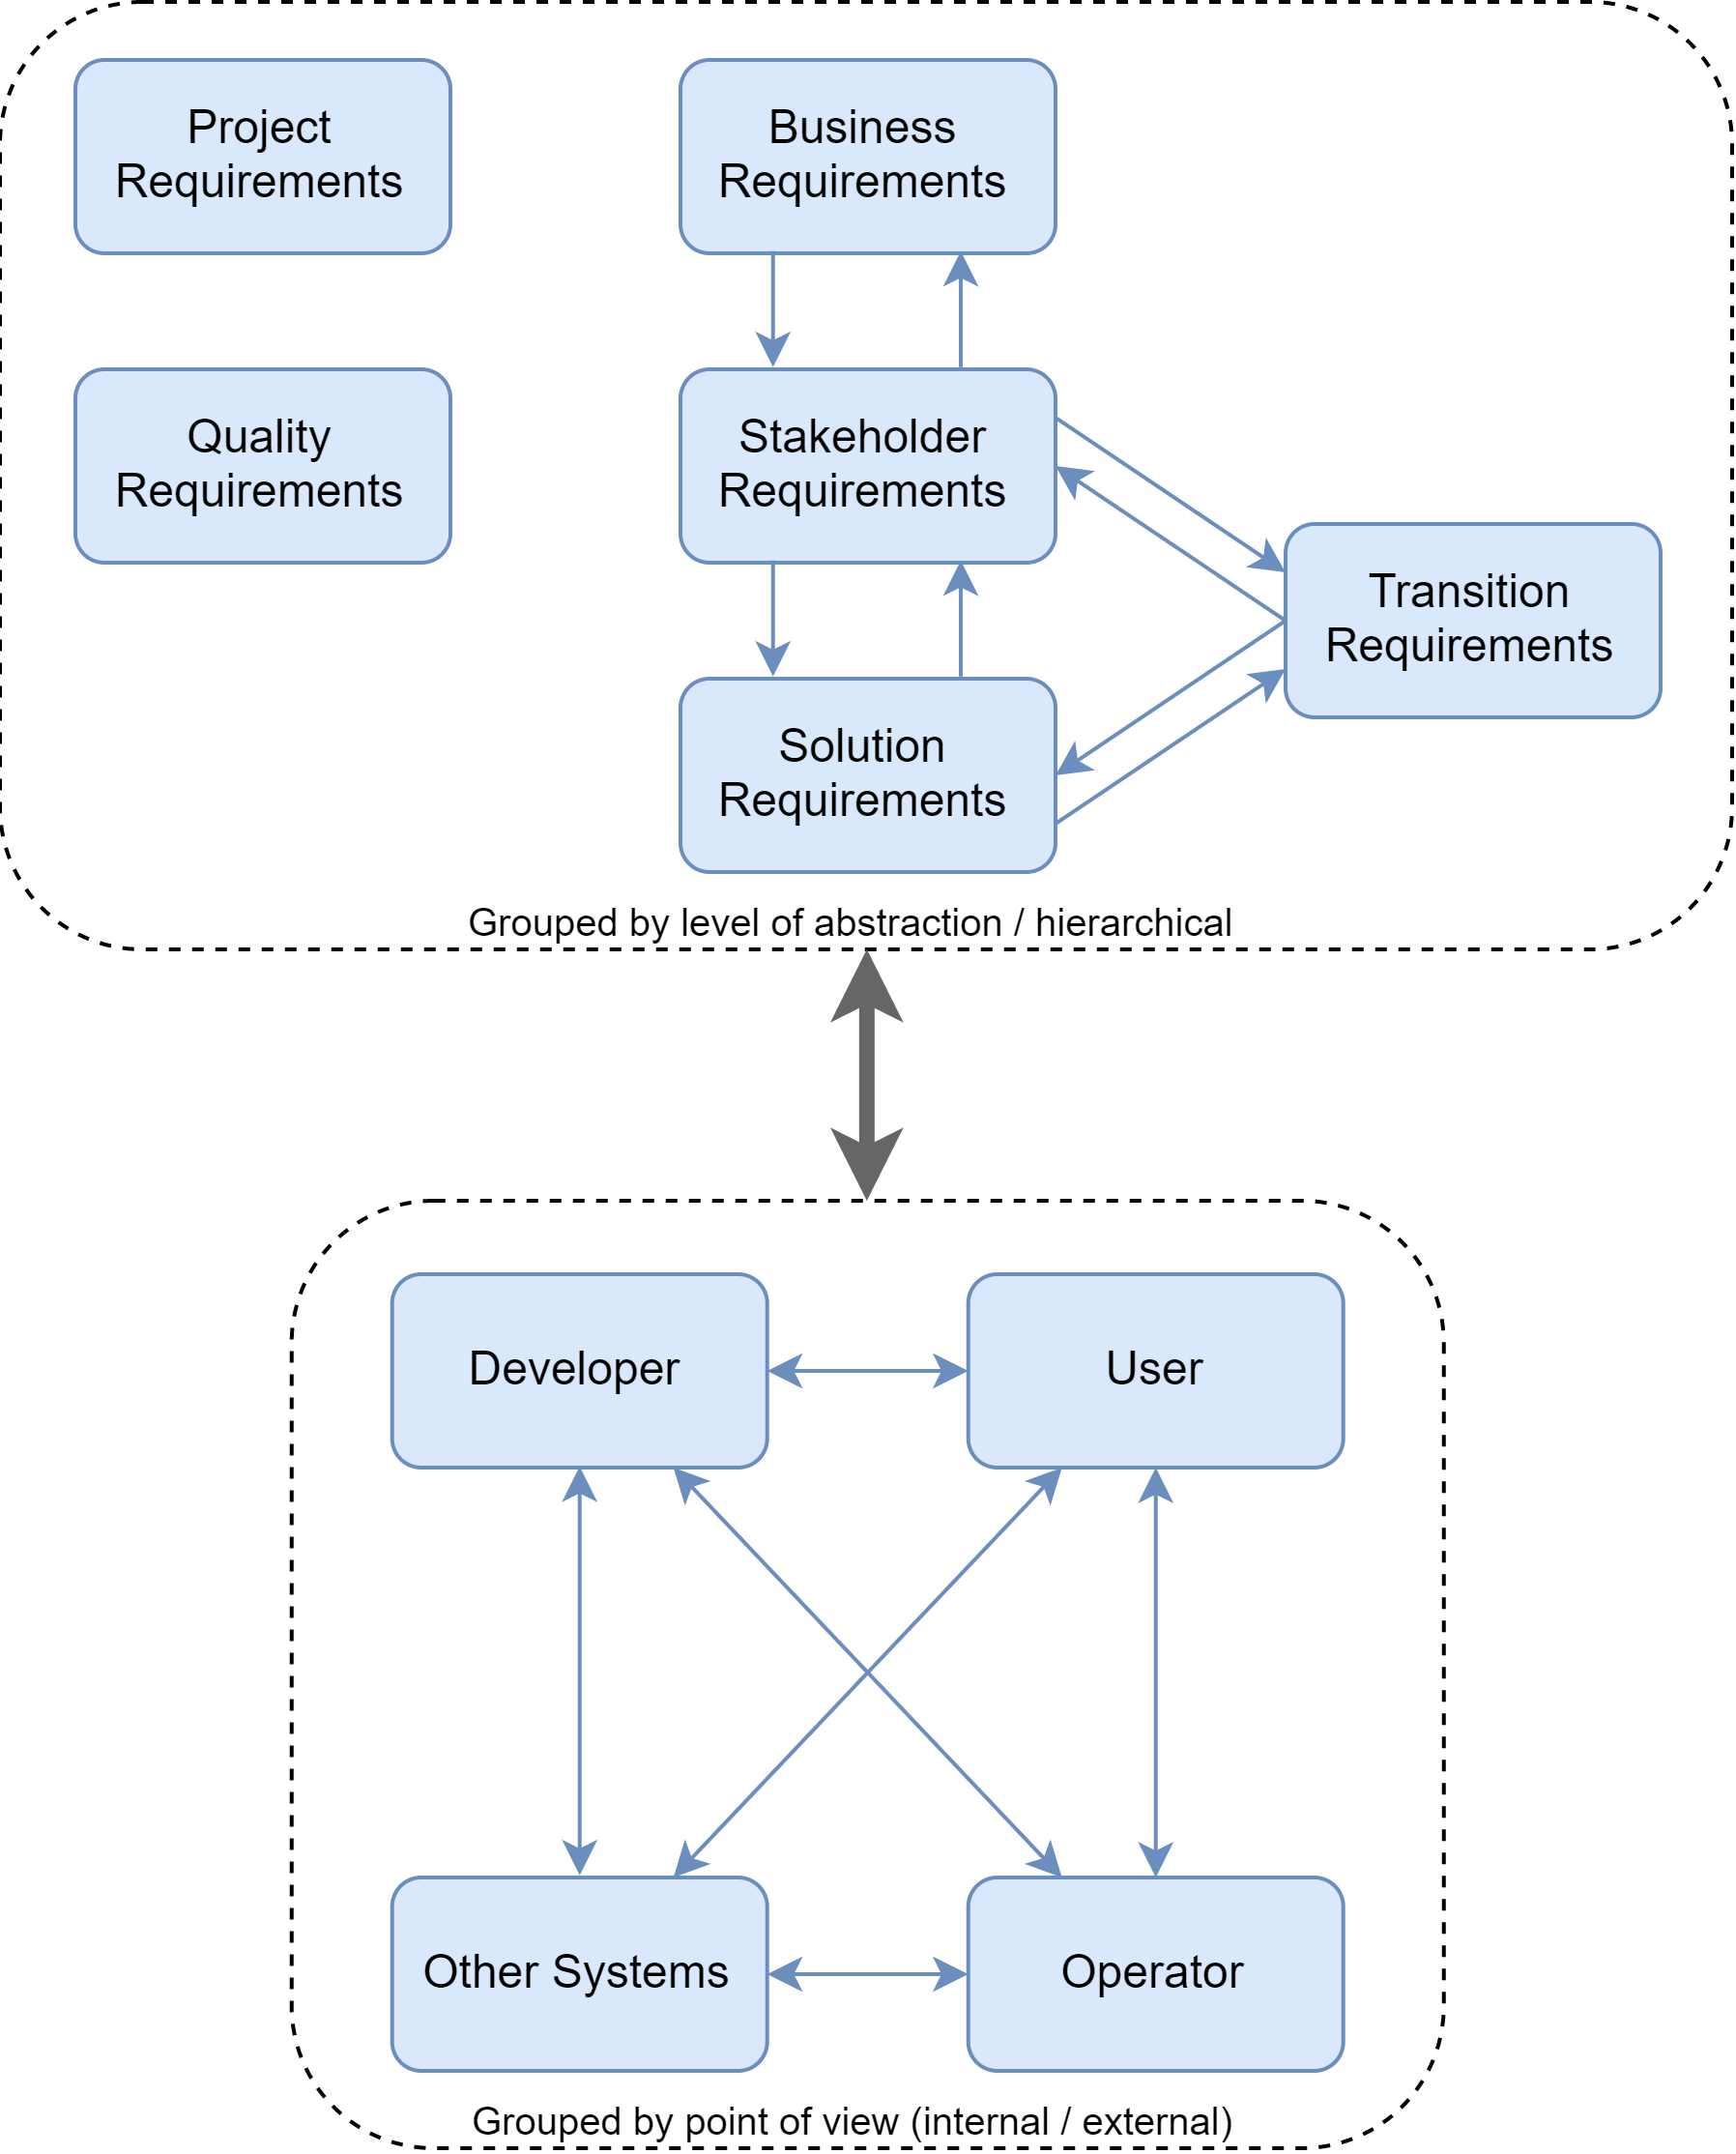
\includegraphics[width=1.0\textwidth]{gfx/Requirements_Grouping.png}
 \caption{Anforderungen werden nach zwei verschiedenen Ansätzen gruppiert.}
 \label{fig:chapter05:requirements_grouping}
\end{figure}

\section{Ableitung eines Klassifizierungsmodells}
\label{sec:requirements:model}

In dieser Arbeit werden die Vorteile mehrerer Ansätze zur Anforderungsklassifizierung kombiniert, indem Anforderungen stufenweise in Unterklassen unterteilt werden. Dabei wurde sich der Klassifizierung des \cite{SWEBOK}, \cite{PMBOK} bzw. \cite{BABOK} und \cite{ISO25010} bedient und die folgende Einordnung erstellt:

\begin{description}
  \item[System Anforderungen] Anforderungen dieser Klasse beziehen sich auf das Gesamtsystem als solches.\\
  Leitfrage: \glqq ? \grqq
  \item[Software Anforderungen] Anforderungen dieser Klasse beziehen sich auf die Softwarekomponente des Gesamtsystems.\\
  Leitfrage: \glqq ? \grqq
  \item[Business Anforderungen] Diese Anforderungen gehören zu der Klasse der System-Anforderungen und beschreiben Anforderungen, die sich an das Geschäftsmodell hinter dem Gesamtsystem richten. Zu dieser Klasse gehören Anforderungen, die sich mit dem Mehrwert für die Organisation beschäftigen und den Nutzen des Gesamtsystems für die Organisation beschreiben.\\
  Leitfrage: \glqq Welche Geschäftsfälle gibt es und wie werden diese abgedeckt? Welche Richtlinien und Vorgaben müssen beachtet werden? \grqq
  \item[Stakeholder Anforderungen] Diese Anforderungen gehören zu der Klasse der System-Anforderungen und beschreiben Anforderungen, die die Interessen der beteiligten Stakeholder widerspiegeln und sich keiner anderen Klasse zuordnen lassen.\\
  Leitfrage: \glqq Was muss das Gesamtsystem aus Sicht von [Stakeholder] können? \grqq
  \item[Transitionsanforderungen] Diese Anforderungen gehören zu der Klasse der System-Anforderungen und beschreiben den Übergang vom IST-Zustand des Systems in den SOLL-Zustand. Beispiele hierfür sind benötigte Anwenderschulungen oder Datenkonvertierungen.\\
  Leitfrage: \glqq Was muss gegeben sein, damit sich das Gesamtsystem von Zustand A nach Zustand B überführen lässt? \grqq
  \item[Projekt Anforderungen] Diese Anforderungen gehören zu der Klasse der System-Anforderungen und beschreiben die Rahmenbedingungen an das Entwicklungsprojekt. Beispiele hierfür können die Projektsprache und etwaige Dokumentationsrichtlinien sein.\\
  Leitfrage: \glqq Welche Rahmenbedingungen sind dem Entwicklungsprojekt gegeben? \grqq
  \item[Qualitätsanforderungen] Als Unterklasse der System-Anforderungen beschreiben die Qualitätsanforderungen die Qualitätsansprüche an das System und die Entwicklung und definieren Akzeptanzkriterien ähnlich zu  \ac{DoR} bzw. \ac{DoD}.\\
  Leitfrage: \glqq Welche Qualitätsansprüche werden an das Gesamtsystem gestellt? \grqq
  \item[Nicht-funktionale Anforderungen] Diese Anforderungen werden gemäß \ac{ISO}-Norm 25010 zur Software-Qualität definiert und sind Teil der Software-Anforderungen. Es wird die Art und Weise beschrieben, wie die Software die gestellten Anforderungen erfüllen soll. Dazu zählen zum Beispiel die Performanz, die Kompatibilität und die Benutzbarkeit. Eine ausführliche Auflistung aller Klassen unter dem Sammelbegriff der nicht-funktionalen Anforderungen sowie die genauen Definitionen der Begriffe kann unter \cite{ISO25010} eingesehen werden. \\
  Leitfrage: \glqq Wie gut muss die Software etwas können? \grqq
  \item[Funktionale Anforderungen] Diese Unterklasse der Software-Anforderungen beschreibt, was das Software-System leisten muss und welche Aufgaben es erfüllen muss.\\
  Leitfrage: \glqq Was muss die Software können? \grqq
  \item[Prozess Anforderungen] Als Untergruppe der Software-Anforderungen bündelt diese Klasse alle Anforderungen, die den Prozess beschreiben, damit die Software so wird wie gefordert. Typischerweise sind Anforderungen an den Softwareentwicklungsprozess enthalten.\\
  Leitfrage: \glqq Was ist beim Entwickeln der Software zu beachten? \grqq
  \end{description}

Die Abbildung \ref{fig:chapter05:requirements_hierarchy} fasst die Anforderungstypen zusammen und stellt sie hierarchisch strukturiert dar. Es wird deutlich, dass das entwickelte Modell beide Sichtweisen (vgl. Abbildung \ref{fig:chapter05:requirements_grouping}) aufgreift. Auf Seite der System-Anforderungen werden verschiedene Abstraktionslevel wie zum Beispiel die Business-Anforderungen und die Stakeholder-Anforderungen unterschieden. Auf der Seite heben die Stakeholder-Anforderungen die Interessen der Beteiligten hervor und betrachten die Anforderungen zusammen mit den Software-Requirements aus unterschiedlichen Perspektiven.

\begin{figure}[htbp]
 \centering
 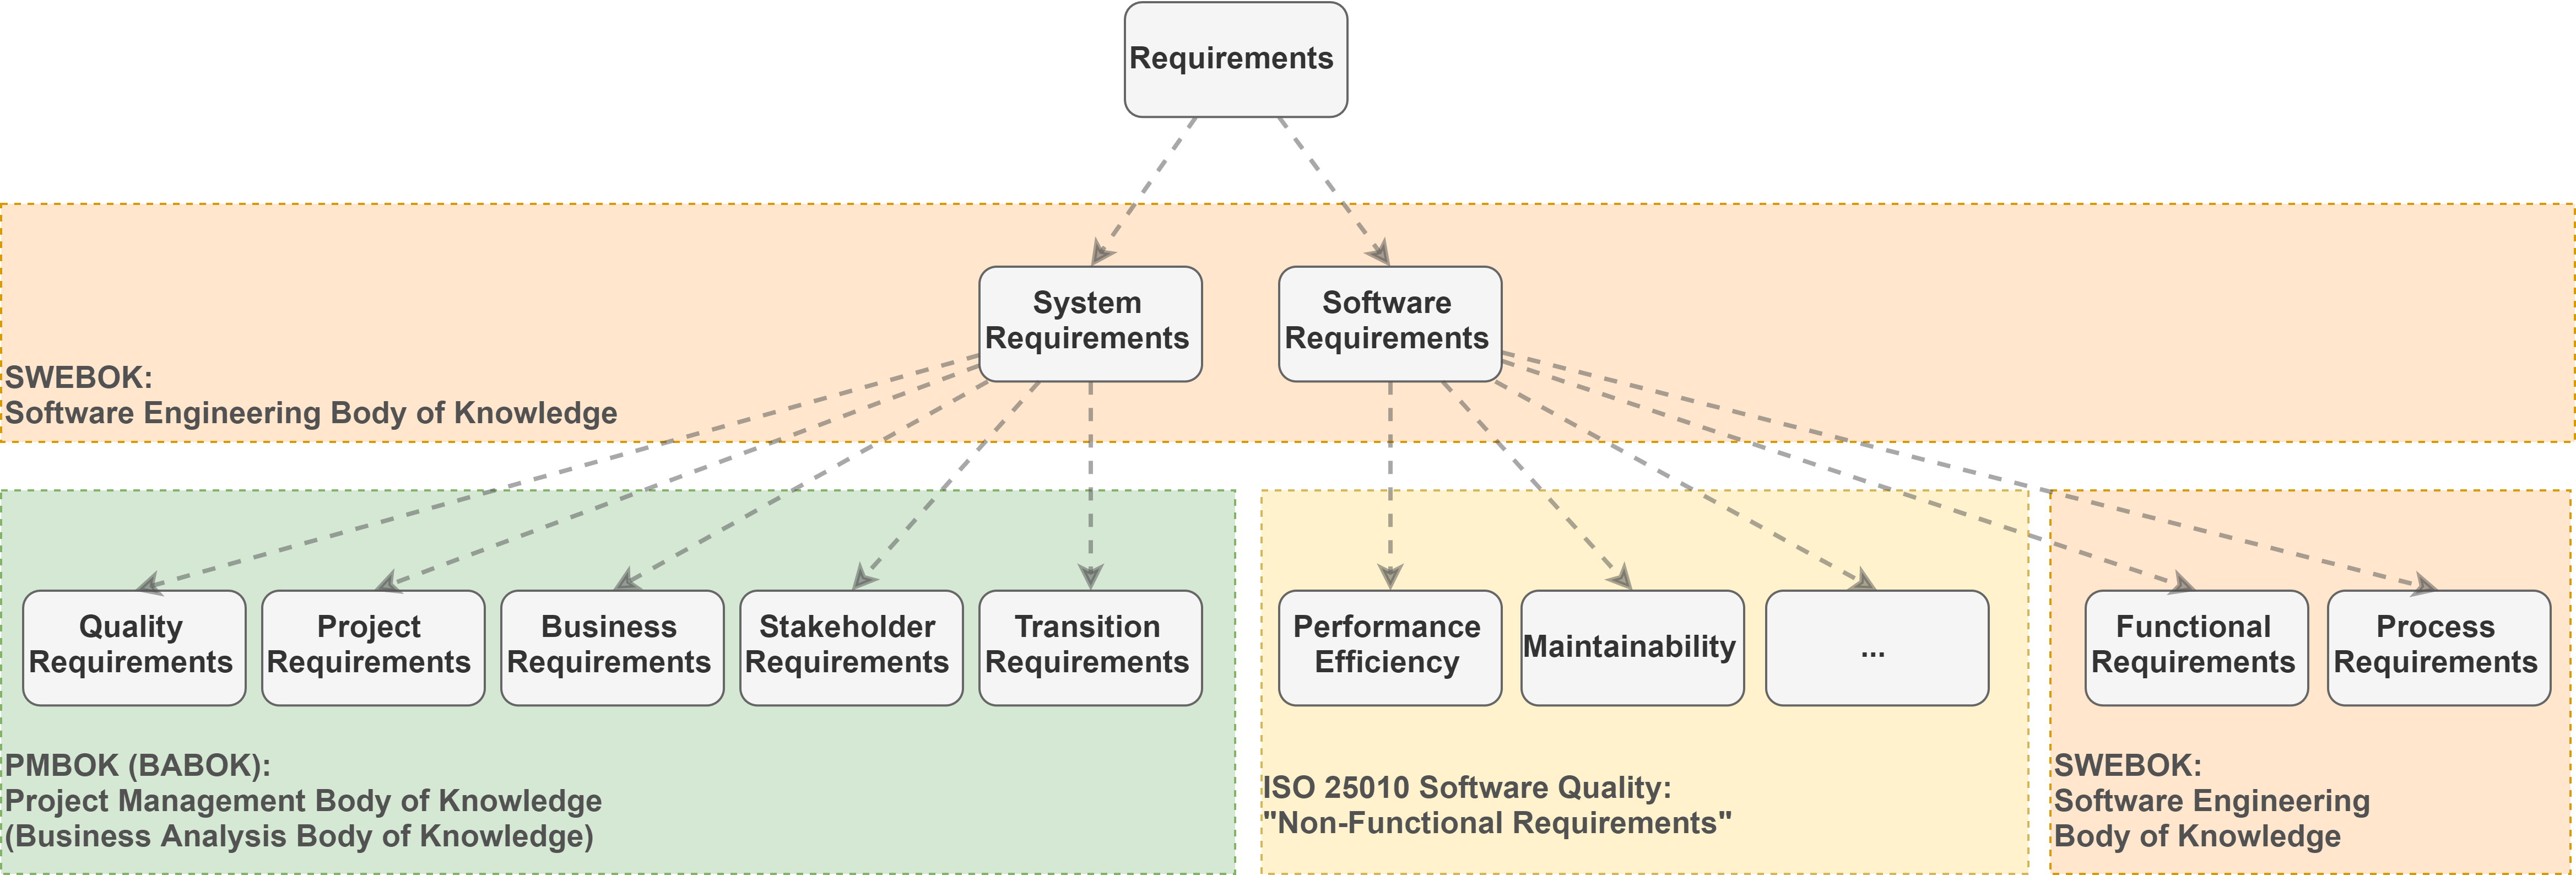
\includegraphics[width=1.0\textwidth]{gfx/Requirements_Hierarchy.png}
 \caption{Anforderungsklassifizierung als kombiniertes Modell aus \cite{SWEBOK}, \cite{PMBOK} bzw. \cite{BABOK} und \cite{ISO25010}}
 \label{fig:chapter05:requirements_hierarchy}
\end{figure}

%
% Section: Anforderungsanalyse
%
\section{Anforderungsanalyse}
\label{sec:requirements:analysis}
In diesem Abschnitt werden die Anforderungen zu dem in Kapitel \ref{ch:iot_usecase} vorgestellten Anwendungsfall ermittelt. Dazu werden zunächst alle beteiligten Stakeholder identifiziert und kurz beschrieben. Anschließend werden aus der jeweiligen Perspektive heraus User-Stories gebildet und die daraus abgeleiteten Tasks aufgelistet. Eine detaillierte Beschreibung aller daraus resultierenden Anforderungen sowie die genaue Zuordnung zu den User-Stories sind im Anhang \ref{ch:appendix:requirements} zu finden.\\

Die Rollen Hersteller, Kunde, Service-Dienstleister und Lieferant wurden bereits unter \ref{description:chapter04:stakeholder} beschrieben. Die folgende Auflistung zeigt weitere Rollen, die über die bereits genannten hinausgehen:
\begin{description}
  \item[Plattform-Betreiber] Der Plattform-Betreiber ist verantwortlich für den Betrieb der Plattform und ist hauptsächlich an einem stabilen System und interessiert.
  \item[IT-Security-Beauftragter] Für den IT-Security-Beauftragten stehen aller sicherheitsrelevanten Themen im Fokus. Dazu zählen insbesondere Verschlüsselung, Datensicherheit und Datenschutz sowie die Authentizität von Daten.
  \item[Business-Developer] Der Business-Developer beschäftigt sich mit der Unternehmensentwicklung und hat Anforderungen an das Geschäftsmodell, die Wirtschaftlichkeit und die Zielerreichung des Gesamtsystems.
  \item[System-Architekt] Für den Software-Architekten stehen alle Fragen rund um die IT-Architektur der Plattform im Vordergrund. Dazu zählen \ac{API}s, Modularisierung und der generelle Aufbau der Software.
\end{description}



%
% Section: Anforderungsklassifizierung
%
\section{Anforderungsklassifizierung}
\label{sec:requirements:classification}
Die zuvor ermittelten Anforderungen werden nach dem Klassifizierungsschema aus Abschnitt \ref{sec:requirements:model} gruppiert. Die Tabelle \ref{tab:requirements_classify} stellt die Einordnung übersichtlich dar.

\begin{table}[h]
    \myfloatalign
    \begin{tabularx}{\textwidth}{Xll} \toprule
        \tableheadline{labitur bonorum pri no} & \tableheadline{que vista}
        & \tableheadline{human} \\ \midrule
        fastidii ea ius & germano &  demonstratea \\
        suscipit instructior & titulo & personas \\
        %postulant quo & westeuropee & sanctificatec \\
        \midrule
        quaestio philosophia & facto & demonstrated \\
        %autem vulputate ex & parola & romanic \\
        %usu mucius iisque & studio & sanctificatef \\
        \bottomrule
    \end{tabularx}
    \caption[Autem usu id]{Autem usu id.}
    \label{tab:requirements_classify}
\end{table}

%
% Section: Anforderungsevaluierung
%
\section{Anforderungsevaluierung}
\label{sec:requirements:evaluation}
Schrittweises Reduzieren der Anforderungen um DLT-relevante Anforderungen zu identifizieren...
